% compile with: pdflatex -shell-escape filename.tex
\documentclass[crop,tikz,convert=pdf2svg]{standalone}
\usepackage{tikz}
\usetikzlibrary{backgrounds}
\usetikzlibrary{calc}
\usetikzlibrary{decorations.pathreplacing}
\usetikzlibrary{matrix}
\usetikzlibrary{positioning}

\tikzset{
  label/.style={
    anchor=west,
    minimum width=60pt,
    text width=60pt,
  },
}

\tikzset{
  ncbar angle/.initial=90,
  ncbar/.style={
    to path=(\tikztostart)
    -- ($(\tikztostart)!#1!\pgfkeysvalueof{/tikz/ncbar angle}:(\tikztotarget)$)
    -- ($(\tikztotarget)!($(\tikztostart)!#1!\pgfkeysvalueof{/tikz/ncbar angle}:(\tikztotarget)$)!\pgfkeysvalueof{/tikz/ncbar angle}:(\tikztostart)$)
    -- (\tikztotarget)
  },
  ncbar/.default=0.5cm,
}

\tikzset{
  bracket/.style={ncbar=-0.25cm}
}

\begin{document}

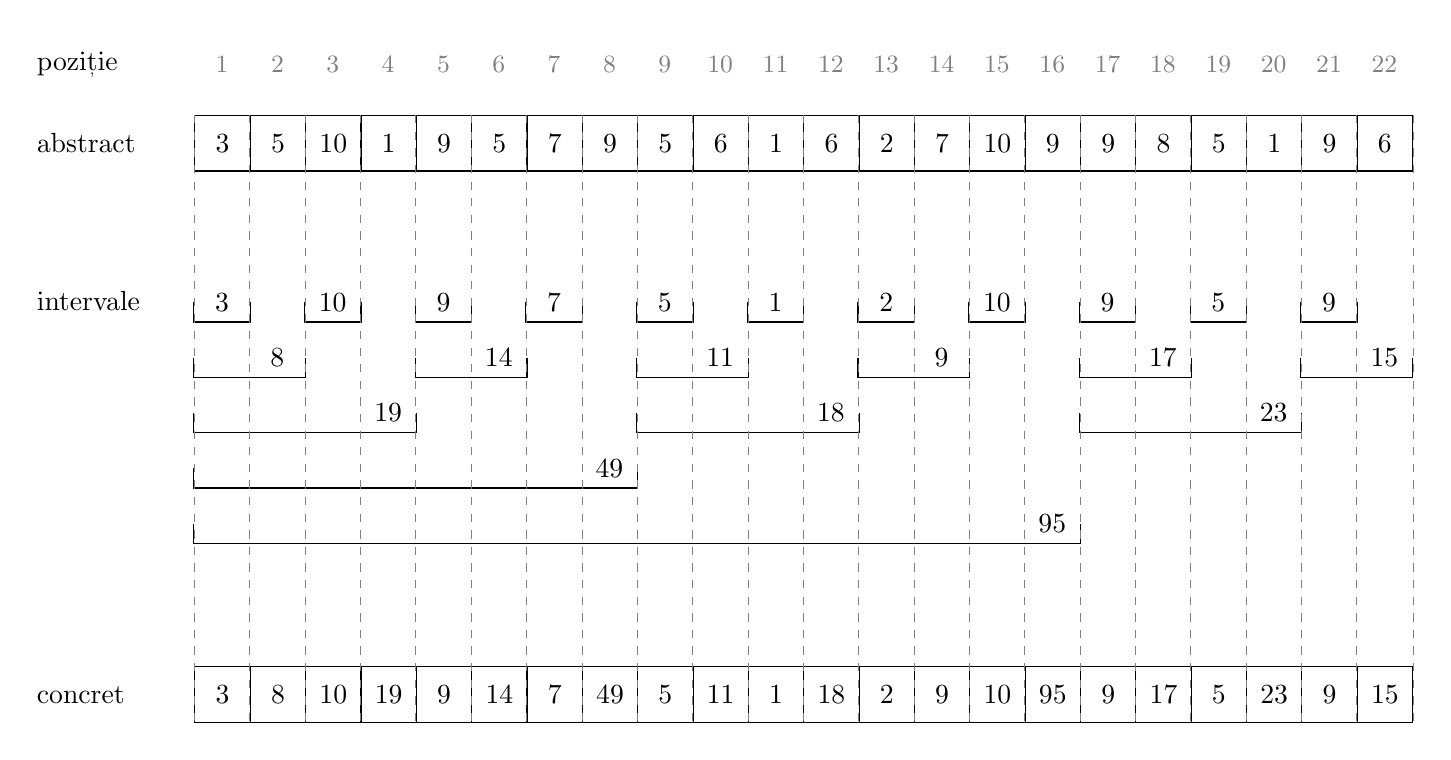
\begin{tikzpicture}
  % First row: indices
  \node[label] (label-index) at (0, 0) {poziție};

  \matrix[right] (index) at (2, 0) [
    matrix of nodes,
    nodes={anchor=center, minimum size=20pt, color=black!50, font=\small},
  ] {
    1 & 2 & 3 & 4 & 5 & 6 & 7 & 8 & 9 & 10 & 11 & 12 & 13 & 14 & 15 & 16 & 17 & 18 & 19 & 20 & 21 & 22\\
  };

  % Second row: abstract values
  \node[label] (label-abstract) at (0, -1) {abstract};

  \matrix[right] (abstract) at (2, -1) [
    matrix of nodes,
    nodes={draw, anchor=center, minimum size=20pt},
    column sep=-\pgflinewidth,
    row sep=-\pgflinewidth
  ] {
    3 & 5 & 10 & 1 & 9 & 5 & 7 & 9 & 5 & 6 & 1 & 6 & 2 & 7 & 10 & 9 & 9 & 8 & 5 & 1 & 9 & 6\\
  };

  % Third row: partial sum intervals
  \node[label] (label-intervals) at (0, -3) {intervale};

  \matrix[below right=-13pt and 0pt] (int) at (2, -3) [
    matrix of nodes,
    nodes={anchor=center, minimum size=20pt},
  ] {
    3 & \  & 10 & \  & 9 & \  & 7 & \  & 5 & \  & 1 & \  & 2 & \  & 10 & \  & 9 & \  & 5 & \  & 9 & \ \\
    \  & 8 & \  & \  & \  & 14 & \  & \  & \  & 11 & \  & \  & \  & 9 & \  & \  & \  & 17 & \  & \  & \  & 15\\
    \  & \  & \  & 19 & \  & \  & \  & \  & \  & \  & \  & 18 & \  & \  & \  & \  & \  & \  & \  & 23 & \  & \ \\
    \  & \  & \  & \  & \  & \  & \  & 49 & \  & \  & \  & \  & \  & \  & \  & \  & \  & \  & \  & \  & \  & \ \\
    \  & \  & \  & \  & \  & \  & \  & \  & \  & \  & \  & \  & \  & \  & \  & 95 & \  & \  & \  & \  & \  & \ \\
  };

  \foreach \x in {1,3,...,21} {
    \draw (int-1-\x.west) to [bracket] (int-1-\x.east);
  }
  \draw (int-2-1.west) to [bracket] (int-2-2.east);
  \draw (int-2-5.west) to [bracket] (int-2-6.east);
  \draw (int-2-9.west) to [bracket] (int-2-10.east);
  \draw (int-2-13.west) to [bracket] (int-2-14.east);
  \draw (int-2-17.west) to [bracket] (int-2-18.east);
  \draw (int-2-21.west) to [bracket] (int-2-22.east);

  \draw (int-3-1.west) to [bracket] (int-3-4.east);
  \draw (int-3-9.west) to [bracket] (int-3-12.east);
  \draw (int-3-17.west) to [bracket] (int-3-20.east);

  \draw (int-4-1.west) to [bracket] (int-4-8.east);

  \draw (int-5-1.west) to [bracket] (int-5-16.east);

  % Fourth row: concrete values
  \node[label] (label-concrete) at (0, -8) {concret};

  \matrix[right] (concrete) at (2, -8) [
    matrix of nodes,
    nodes={draw, anchor=center, minimum size=20pt},
    column sep=-\pgflinewidth,
    row sep=-\pgflinewidth
  ] {
    3 & 8 & 10 & 19 & 9 & 14 & 7 & 49 & 5 & 11 & 1 & 18 & 2 & 9 & 10 & 95 & 9 & 17 & 5 & 23 & 9 & 15\\
  };

  % Vertical grid lines
  \foreach \x in {1,...,22} {
    \draw [help lines, dashed] (abstract-1-\x.north west) -- (concrete-1-\x.south west);
  }
  \draw [help lines, dashed] (abstract-1-22.north east) -- (concrete-1-22.south east);

\end{tikzpicture}

\end{document}
